\chapter{Background}

\todo{Assigned Johan L}

% WHAT IS A COMPILER 

The Erlang virtual machine is appreciated for its excellent support for
concurrency, distribution and error handling, allowing soft-real-time systems
with high uptimes - famously demonstrated by the 99.9999999\% uptime of
Ericsson’s AXD301 telecom switch from 1998. The features of the BEAM (Erlang’s
main virtual machine implementation) aren't tied to Erlang itself: one can
enjoy the benefits of the runtime with a different syntax and semantics.
Previous efforts in this field include: Elixir, a language with Ruby-like
syntax; Javascript flavoured Erlang, Lisp flavoured Erlang and a YHC Haskell
to Erlang transpiler that preserves laziness.

Attempts to port Erlang features to Haskell have also been made, illustrating
the demand for a combination of the languages’ features. Cloud Haskell is
‘Erlang in a library’, but differences in the Erlang and Haskell runtime
system make shipping expressions between nodes far more verbose than in Erlang.

Haskell is known for its terse and elegant syntax, in addition to a powerful
type system that prevents many programming errors and makes it easier to
reason about code. Erlang developers already use code analysis tools to write
typed code, but these tools don’t interact well with message passing where the type received can be hard to predict. Combining the compile-time features of Haskell with the run-time benefits of Erlang into a language interoperable with the latter would be a great boon for Erlang developers.

%To take advantage of both BEAM's great concurrency model with the safety of 
%Haskell's typesystem this project is intended to design and implement a new 
%language named Hopper.  

New languages are often developed to allow for a higher level of abstraction and a higher level of reasoning about algorithms. To be able to run these new languages compilers are built to convert the high level code down to machine code, to run directly on hardware, or to a lower level language to make use of that language's compiler. 

% GENERAL PIPELINE FIGURE

\todo{Update figure: Typechecker -> Type checker}

\begin{figure}[h!]
  \centering
  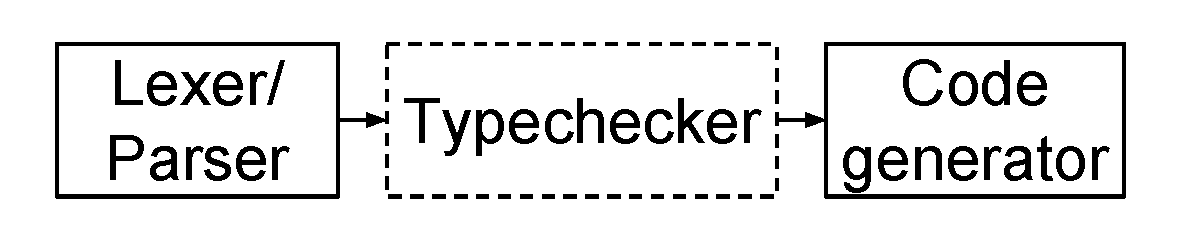
\includegraphics[width=0.6\pdfpagewidth]{figure/general-pipeline}
  \caption{A general compiler pipeline}
  \label{fig:generalpipeline}
\end{figure}

% HOW IS A COMPILER BUILT 

The structure of a compiler can be likened to a pipe where text flows through. 
The text flowing through the pipe is transformed between different representations and is in
the end output as runnable code to either run on the computer itself or on a virtual machine
that emulates a computer. 

In figure ~\ref{fig:generalpipeline} you can see the flow handling the source code.
It should be noted that the type checker is optional for a language, it can
fully rely on the grammar to expose errors. This will lead to a more expressive, 
or less restricted, language but increases the risk of runtime crashes due to type errors.

We start by describing the first step of a compiler, the lexer and parser.

%Now is Hopper really a transpiler or a translating compiler. Instead of 
%outputting runnable code it outputs other code that is interpreted and compiled
%by the Erlang compiler, erlc. With this the project could very much be 
%simplified (ref to read more in discussion).


% OTHER SECTIONS

\section{Parsing source code} \label{sec:bnfc}

\todo{Assigned David}


A programming language is similar to a natural language in that it is described by a grammar. Programming languages are however different in that they are built from their grammar and are thus unambiguous.
The grammar describes ways in which the smaller pieces of the language can be put together to form bigger ones, often with more meaning. 

From this grammar a lexer is produced. The lexers job is to match all words in the source code to tokens in the grammar. For example in english the word 'boat' would match a noun token. This list of tokens is combined with a parser to make expressions or sentences. To make the language as expressive as possible one build up bigger expressions out of smaller expressions. This will create a tree structure that will be easier to work with. 

To save a lot of work, the lexer and parser can be automatically generated from a grammar written in \gls{bnf} using a tool called the \gls{bnfc} \cite{bnfc}, or BNFC for short. This tool is developed at Chalmers and used in earlier courses, meaning that multiple group members were already familiar with it.
\section{Renaming and simplifying}

\todo{Assigned DAvid}

While BNFC is a great tool to create a parse tree from raw text the resulting 
tree structure is very verbose with a lot of constructors. To simplify this a
renamer step is introduced in the pipeline. This step converts the parse tree
to our minimally designed \acrlong{ast} or \acrshort{ast} for short. 

% TODO I want these beside each other and a arrow in between
\begin{table}
\begin{lstlisting} 
f = if a                      f = case a of
      then b        =>              True  -> b
      else c                        False -> c
\end{lstlisting}
\caption{Simple transformation to a more general form}
\label{lst:renamer1}
\end{table}

In this step a few grammar rules could be translated to more general expressions
to simplify the AST and reduce the number of cases the typechecker need to cover, see
table \ref{lst:renamer1}.

The other part of the renamer module is to annotate the functions to where they
where exported from...

\section{Dependency checking}

\todo{Assigned Jakob}

As computer programs increase in complexity, a need for separation of concerns arises. Programming languages typically solve this problem by having a concept of \emph{modules} (sometimes also known as \emph{packages}), cohesive units of code. Besides the organizational benefits, there are technical merits to modular software as well. If a single module is changed, the entire project doesn't necessarily have to be recompiled -- only the parts which \emph{depend} on the module that was changed.

The concept of \emph{dependency} is central in module systems. Most\todo{sources} languages require dependencies between modules to be explicitly declared (e.g. with \texttt{import} statements or similar), but concepts differ between different languages. For example, some languages allow cyclical intermodule dependencies while others forbid it. \todo{fill out, how is it done in other languages?}
\section{Semantic analysis}

An important design decision to make when implementing a programming language is whether to perform some semantic analyses of the code at compile time and what to include in such case. Semantic analyses can for example contribute error detection and optimized code. The cost is increased complexity of the compiler and for some kinds of analysis prohibitive compilation times.

A common and well studied category of analyses is type inference or type checking. Type systems vary in their expressiveness but essentially allow us to prove desireable properties of our code.

\todo{Motivation of Hopper is to bring type checking to erlang}

\todo{What we want from the type system}

\subsection{Type inference}

\todo{Choice of type system}

\todo{Constraint generation by means of inference rules}

\todo{Constraint solving}

\todo{Reporting type results}

%------------------

%what
%  in general
%    a step in the compilation process
%    examine details of the code which cannot be captured be the grammar itself.
%    example control flow analysis
%  type inference
%    a formal system
%    system F in Haskell
%    we use Hindley-Milner type system to begin with

%why
%  in general
%    prove properties
%    show correctness/show absence of errors
%  type inference
%    tractable
%    well established

%how
%  preprocess
%    the simple language
%      lambda calc
%        expressiveness etc
%        extensions (let, fix)
%    transformations
%      parse -> AST ?
%      AST -> simple language
%      important: keep semantics
%  type inference
%    generating constraints by inference rules
%    solving constraints by solving rules
%  postprocess
%    looking upp the solved types and reporting them

\section{Core Erlang and BEAM}

Core Erlang \cite{CoreErlangIntro} is an intermediate language in the Erlang compilation suite, mainly used for simplifying operations on Erlang source code. Such operations can include, but are not limited to: parsing, compiling and debugging. Some of the main purposes of Core Erlang are to be as regular as possible and to provide clear and simple semantics. The language is since release 8, released in 2001, an official part of the OTP/Open Source Erlang Distribution.

\Gls{beam} is the name of the Erlang virtual machine. Erlang and Core Erlang source code may be compiled to \texttt{.beam} files, which contain assembler instructions for the \gls{beam} virtual machine. These instructions are interpreted by the virtual machine at run time.

